% Reporte del Proyecto Apertura 2026B — DBSCAN para detección de ruido con OpenMP
% Compilación: ver entrega/reporte/README.md (tectonic, xelatex o pdflatex; las figuras están en figuras/).
\documentclass[11pt,letterpaper]{article}

\usepackage{iftex}
\ifPDFTeX
  \usepackage[T1]{fontenc}
  \usepackage[utf8]{inputenc}
  \usepackage{lmodern}
\else
  \usepackage{fontspec}
\fi
\usepackage[spanish,es-nodecimaldot,es-tabla,es-noshorthands]{babel}
\usepackage[letterpaper,margin=2.0cm,top=1.8cm,bottom=2.0cm]{geometry}
\usepackage{amsmath,amssymb}
\usepackage{graphicx}
\usepackage{booktabs,tabularx,array}
\usepackage{xcolor}
\usepackage{tikz}
\usepackage[font=small,labelfont=bf,skip=3pt]{caption}
\usepackage{enumitem}
\usepackage{listings}
\usepackage{titlesec}
\usepackage{microtype}
\usepackage[hidelinks]{hyperref}
\makeatletter\g@addto@macro\UrlBreaks{\do\_}\makeatother

\titlespacing*{\section}{0pt}{9pt plus 2pt minus 1pt}{4pt}
\titlespacing*{\subsection}{0pt}{6pt plus 2pt minus 1pt}{2pt}
\titlespacing*{\paragraph}{0pt}{4pt plus 1pt minus 1pt}{0.7em}
\titleformat{\section}{\large\bfseries}{\thesection.}{0.5em}{}
\titleformat{\subsection}{\normalsize\bfseries}{\thesubsection.}{0.5em}{}
\setlist{itemsep=0pt,topsep=2pt,parsep=0pt,leftmargin=1.2em}
\setlength{\parskip}{1pt}
\setlength{\textfloatsep}{8pt plus 2pt minus 2pt}
\setlength{\floatsep}{6pt plus 2pt minus 2pt}
\setlength{\abovedisplayskip}{4pt plus 2pt minus 1pt}
\setlength{\belowdisplayskip}{4pt plus 2pt minus 1pt}
\renewcommand{\topfraction}{0.9}
\renewcommand{\textfraction}{0.08}

\definecolor{pone}{HTML}{2A78D6}
\definecolor{ptwo}{HTML}{C4501F}
\definecolor{halo}{HTML}{F7D3BF}
\definecolor{tinta}{HTML}{52514E}

\newcommand{\code}[1]{\texttt{#1}}
\newcommand{\pendiente}[1]{\textcolor{red}{\textbf{[#1]}}}
\newcommand{\Tser}{\overline{T}_{\mathrm{serial}}}
\newcommand{\smax}{s_{\text{máx}}}

\lstset{
  language=C++, basicstyle=\ttfamily\footnotesize, columns=fullflexible, keepspaces=true,
  keywordstyle=\color{pone!80!black}\bfseries, commentstyle=\color{tinta}\itshape,
  morekeywords={pragma,omp,parallel,schedule,shared,default,static,dynamic},
  frame=lines, framerule=0.4pt, rulecolor=\color{tinta!40}, xleftmargin=0.5em, aboveskip=4pt, belowskip=2pt,
  literate={á}{{\'a}}1 {é}{{\'e}}1 {í}{{\'i}}1 {ó}{{\'o}}1 {ú}{{\'u}}1 {ñ}{{\~n}}1
}
\renewcommand{\lstlistingname}{Listado}

\hypersetup{pdftitle={Detección de ruido mediante DBSCAN con OpenMP},
            pdfsubject={Proyecto Apertura, Cómputo Paralelo y en la Nube, ITAM}}

\begin{document}

%======================================================================================================
\begin{center}
{\Large\bfseries Detección de ruido mediante DBSCAN:\\[1pt]
comparación de una implementación serial y dos estrategias paralelas con OpenMP\par}
\vspace{0.5em}
{\small Proyecto Apertura \textperiodcentered{} Cómputo Paralelo y en la Nube \textperiodcentered{}
Instituto Tecnológico Autónomo de México (ITAM), Otoño 2026\\
Profesor: Dr.\ J.\ Octavio Gutiérrez García \quad\textperiodcentered\quad 20 de octubre de 2026\\
Integrantes: Mario \pendiente{apellidos} \quad\textperiodcentered\quad \pendiente{nombre completo del segundo
integrante}\par}
\end{center}

\begin{abstract}
\noindent Implementamos en C++ el detector de ruido de dos pasos basado en DBSCAN visto en clase
($\varepsilon=0.03$, \code{min\_samples}~$=10$) en tres versiones: una serial de búsqueda exhaustiva; P1, que
reparte los puntos entre hilos de OpenMP; y P2, que divide el plano en $k$ regiones con halos de ancho
$\varepsilon$. Evaluamos 2,320 ejecuciones (ocho tamaños de 20,000 a 200,000 puntos; 1, 6, 12 y 24 hilos;
$k$ de 2 a 64; diez repeticiones) en un Apple M4 Pro de 12 núcleos. Todas reprodujeron exactamente las clases y
los conteos de vecinos de la versión serial. Con 200,000 puntos y 12 hilos, P1 fue 8.29 veces más rápido que la
versión serial y P2 con $k=64$, 47.77 veces. La ventaja de P2 combina una ganancia algorítmica de 7.83, por
evaluar menos pares, con una ganancia paralela de 6.10; con $k\le 4$, en cambio, P2 fue más lento que P1.
\end{abstract}

%======================================================================================================
\section{Problema y formulación matemática}\label{sec:problema}

El enunciado pide detectar ruido en una nube de puntos del plano con la variante ``ingenua'' de DBSCAN vista en
clase~\cite{enunciado,ester1996}. A diferencia del DBSCAN completo, no se forman ni se numeran grupos: cada punto
recibe una de tres clases mediante dos pasos. Sea $P=\{p_1,\dots,p_N\}$ con $p_i=(x_i,y_i)\in\mathbb{R}^2$, y sean
$\varepsilon=0.03$ y $m=\code{min\_samples}=10$ (los parámetros de todas las ejecuciones oficiales, según el
manifiesto del experimento). El vecindario
\begin{equation}\label{eq:vecindario}
  \mathcal N_\varepsilon(i)=\bigl\{\,j\in\{1,\dots,N\}:\ \lVert p_i-p_j\rVert_2\le\varepsilon\,\bigr\}
\end{equation}
incluye al propio $i$ (a distancia 0) y a los duplicados, igual que scikit-learn~\cite{sklearn}. Las clases son
\begin{align}
  \text{Paso 1 (core de primer grado):}\quad & C_1=\bigl\{\,i:\ |\mathcal N_\varepsilon(i)|\ge m\,\bigr\},
    \label{eq:c1}\\
  \text{Paso 2 (core de segundo grado):}\quad & C_2=\bigl\{\,i\notin C_1:\ \exists\, j\in C_1\ \text{con}\
    j\in\mathcal N_\varepsilon(i)\,\bigr\}, \label{eq:c2}\\
  \text{Ruido:}\quad & R=\{1,\dots,N\}\setminus(C_1\cup C_2), \label{eq:ruido}
\end{align}
codificadas como 1 ($C_1$, el ``core'' de la literatura), 2 ($C_2$, el punto ``borde'') y 0 (ruido). El Paso~2 es de
un solo salto: \eqref{eq:c2} solo consulta $C_1$, que está completo antes de empezar. Un punto de $C_2$ nunca
convierte a otro en $C_2$; no hay la propagación recursiva con la que el DBSCAN completo expande sus grupos.

\paragraph{Distancia al cuadrado.} Como $\varepsilon>0$ y $t\mapsto t^2$ es estrictamente creciente en
$[0,\infty)$,
\begin{equation}\label{eq:cuadrado}
  \lVert p_i-p_j\rVert_2\le\varepsilon \iff (x_i-x_j)^2+(y_i-y_j)^2\le\varepsilon^2 ,
\end{equation}
así que el programa compara distancias al cuadrado y nunca calcula raíces. En doble precisión, los pares a distancia
casi exactamente $\varepsilon$ (frecuentes con tres decimales) los decide el redondeo; por eso las tres versiones usan
una única función (\code{within\_eps}, Listado~\ref{lst:kernel}), compilada sin \code{-ffast-math} ni fusión de
multiplicación y suma (\code{-ffp-contract=off}), y toman las mismas decisiones.

\paragraph{Entrada y salida.} La entrada es el CSV sin encabezado de la libreta \code{DBSCAN\_noise.ipynb}
(\code{x,y} por línea). Con \code{--output} el programa escribe \code{x,y,etiqueta} en el orden de entrada (1 = no
ruido, 0 = ruido, como \code{np.where(clusters==-1, 0, 1)}), que grafica la segunda celda de la libreta; con
\code{--detailed-output}, \code{x,y,clase,conteo}; y en la salida estándar, una línea \code{METRICS} con tiempos y
huellas digitales (FNV-1a de 64 bits) de las clases y los conteos.

%======================================================================================================
\section{Implementaciones: Serial, P1 y P2}\label{sec:impl}

Las tres versiones están en \code{src/dbscan.cpp} (\code{--mode serial|p1|p2}) y comparten el predicado y dos
núcleos (Listado~\ref{lst:kernel}): \code{count\_neighbors} cuenta, sin salida anticipada, los candidatos a distancia
$\le\varepsilon$, y \code{has\_core\_neighbor} indica si alguno de $C_1$ lo está y se detiene en el primero. Solo
difieren en \emph{qué candidatos} recibe cada consulta y \emph{qué hilo} la ejecuta. Ninguna guarda una matriz de
distancias (con $N=200{,}000$ ocuparía 320\,GB); la memoria es $O(N)$. Los resultados se escriben por índice original
en \code{count}, \code{is\_core} y \code{label}, con banderas \code{unsigned char}: un \code{std::vector<bool>}
guarda ocho banderas por byte y haría que dos hilos escribieran el mismo byte.

\begin{lstlisting}[caption={Predicado y núcleo del Paso 1, compartidos por las tres versiones.},label={lst:kernel}]
inline bool within_eps(double dx, double dy, double eps2) {   // eps2 = eps * eps
    return dx * dx + dy * dy <= eps2;
}
int count_neighbors(double xq, double yq, const double* xs, const double* ys, int n, double eps2) {
    int count = 0;           // el punto consultado es uno de los candidatos: se cuenta a sí mismo
    for (int j = 0; j < n; j++)
        if (within_eps(xs[j] - xq, ys[j] - yq, eps2)) count++;
    return count;
}
\end{lstlisting}

\subsection{Serial: búsqueda exhaustiva}
\code{dbscan\_serial} hace dos recorridos secuenciales: el Paso~1 cuenta los vecinos de cada $i$ entre los $N$
puntos y marca \code{is\_core[i]}; ya con todas las banderas, el Paso~2 asigna 1, 2 (si \code{has\_core\_neighbor}
encuentra un punto de $C_1$) o 0. El Paso~1 evalúa exactamente $N^2$ veces el predicado: el costo es $O(N^2)$. El
Paso~2 casi no cuesta con nuestros datos (3\,ms de 8.68\,s con $N=200{,}000$) porque casi todos los puntos están en
$C_1$. Serial no usa regiones ni directivas de OpenMP (solo \code{omp\_get\_wtime()} para medir), y el programa
rechaza \code{--k} y cualquier \code{--threads} distinto de 1.

\subsection{P1: paralelización por puntos (``toda la matriz indivisible'')}
P1 conserva la búsqueda exhaustiva y reparte las iteraciones externas entre hilos (Listado~\ref{lst:p1}): cada hilo
clasifica puntos distintos y todos leen el arreglo completo. \code{schedule(static)} divide el ciclo desde el inicio
en bloques contiguos de unas $N/T$ iteraciones, sin costo de reparto; es razonable porque cada iteración recorre los
mismos $N$ candidatos. Se eligió con una medición previa (decisión D4): \code{dynamic,64} fue un 5\,\% más rápido
con 12 hilos, pero sin superar el umbral fijado de antemano (dos desviaciones estándar), y la regla eligió la opción
más simple.

El Paso~2 es otro \code{parallel for} que lee \code{is\_core} y escribe \code{label[i]}; la barrera implícita al
final del primer ciclo garantiza que $C_1$ está completo. No hay condiciones de carrera: cada posición $i$ de
\code{count}, \code{is\_core} y \code{label} la escribe solo su iteración, sin \code{critical}, \code{atomic} ni
candados. Antes de medir, \code{start\_threads} llama a \code{omp\_set\_dynamic(0)} (impide usar menos hilos de los
pedidos; no es \code{schedule(dynamic)}) y crea el equipo de hilos. P1 sigue evaluando los $N^2$ pares, solo que
repartidos entre $T$ hilos.

\begin{lstlisting}[caption={Paso 1 de P1. Cada iteración escribe únicamente las posiciones de su punto.},label={lst:p1}]
#pragma omp parallel for default(none) \
        shared(n, x, y, count, is_core, eps2, min_samples) schedule(static)
for (int i = 0; i < n; i++) {
    count[i]   = count_neighbors(x[i], y[i], x, y, n, eps2);   // todos los puntos son candidatos
    is_core[i] = count[i] >= min_samples;
}   // barrera implícita: ningún hilo empieza el Paso 2 antes de que is_core esté completo
\end{lstlisting}

\subsection{P2: regiones del plano con halos (``dividir la matriz por \texorpdfstring{$k$}{k}'')}\label{sec:p2}
\begin{figure}[t]
\begin{minipage}[c]{0.47\textwidth}\centering
\begin{tikzpicture}[x=0.72cm,y=0.72cm,font=\small]
  \def\e{0.55}
  \fill[halo] (4,0) rectangle (4+\e,2.5+\e);
  \fill[halo] (0,2.5) rectangle (4,2.5+\e);
  \draw[tinta!70,line width=0.5pt] (4,0) -- (4,5) (0,2.5) -- (8,2.5);
  \draw[tinta,line width=0.8pt] (0,0) rectangle (8,5);
  \node[tinta] at (0.5,0.45) {$R_0$}; \node[tinta] at (7.5,0.45) {$R_1$};
  \node[tinta] at (0.5,4.55) {$R_2$}; \node[tinta] at (7.5,4.55) {$R_3$};
  \foreach \p in {(1.3,1.4),(2.2,0.9),(2.5,1.5),(3.3,0.7),(1.7,2.0)} \fill[black] \p circle (1.4pt);
  \draw[pone,line width=0.7pt] (3.75,2.2) circle (\e);
  \fill[pone] (3.75,2.2) circle (1.7pt);
  \node[pone] at (2.93,2.2) {$p_i$};
  \fill[ptwo] (4.12,2.58) circle (1.7pt) node[right=1pt,yshift=3pt] {$p_j$};
  \foreach \p in {(4.3,1.2),(4.4,0.4),(2.0,2.85),(0.6,2.7)} \fill[ptwo] \p circle (1.4pt);
  \foreach \p in {(6.3,0.6),(5.6,3.6),(6.9,3.0),(2.6,4.0)} \draw[tinta] \p circle (1.4pt);
  \draw[tinta,->,line width=0.4pt] (5.15,1.55) -- (4.62,1.55);
  \node[tinta,anchor=west,align=left,font=\footnotesize] at (5.2,1.55) {halo de $R_0$\\(ancho $\varepsilon$)};
\end{tikzpicture}
\end{minipage}\hfill
\begin{minipage}[c]{0.5\textwidth}
\caption{P2 con $k=4$. La región $R_0$ compara sus puntos propios (negro) con ellos mismos y con los de su halo
(naranja): la franja sombreada de ancho $\varepsilon$ en las regiones vecinas, incluida la esquina diagonal. El
vecino $p_j$ de $p_i$ pertenece a $R_3$, pero está en el halo de $R_0$. Los puntos huecos nunca se comparan con los
de $R_0$: ese es el ahorro de trabajo de P2.}
\label{fig:halo}
\end{minipage}
\end{figure}

P2 divide la caja envolvente en $k=r\times c$ rectángulos iguales ($r$: el mayor divisor de $k$ que no supera
$\sqrt k$; $k=2$: mitades verticales, $k=4$: cuadrantes, $k=64$: $8\times8$), como en el dibujo del enunciado. La
\textbf{región propietaria} de $i$ es la celda que contiene a $p_i$; la asigna \code{strip\_index}, que nunca
disminuye cuando la coordenada crece, así que cada punto tiene una sola dueña. El \textbf{halo} de la región $r$ son
los puntos de otras regiones a distancia $\le\varepsilon$ de su rectángulo en cada eje, incluidas las diagonales
(Figura~\ref{fig:halo}): cada punto $j$ entra al halo de todas las regiones que toca el cuadrado
$[x_j-\mu,x_j+\mu]\times[y_j-\mu,y_j+\mu]$, con $\mu=\varepsilon+10^{-9}(M+\varepsilon)$ y $M$ la mayor coordenada
en valor absoluto (el margen, $\approx10^{-9}$, solo absorbe redondeo). La \textbf{lista local de candidatos} $L_r$
tiene los $n_r$ puntos propios seguidos del halo, copiados a arreglos contiguos con su índice original.

\paragraph{Por qué el halo no pierde vecinos.} Como $|x_i-x_j|\le\sqrt{(x_i-x_j)^2+(y_i-y_j)^2}$, y lo mismo en $y$,
\begin{equation}\label{eq:halo}
  \lVert p_i-p_j\rVert_2\le\varepsilon \;\Longrightarrow\; |x_i-x_j|\le\varepsilon\ \ \text{y}\ \
  |y_i-y_j|\le\varepsilon .
\end{equation}
Entonces $x_j-\mu\le x_i\le x_j+\mu$; como \code{strip\_index} es monótona y es la \emph{misma} función que define
la región propietaria, la columna de la región de $i$ está en el rango que alcanza $j$, e igual con las filas: todo
vecino real de un punto propio está en $L_r$. Cada punto aparece una sola vez en $L_r$ y los candidatos de más se
descartan con el predicado exacto~\eqref{eq:cuadrado}, así que los conteos son idénticos a los de Serial (la
demostración con redondeo, válida en el dominio numérico que el programa acepta, está en la decisión D5).

\paragraph{Fases.} (i) \emph{Construcción} (\code{t\_build}): caja, región propietaria y alcance de cada punto, y
listas $L_r$ (trabajo $O(kN)$). (ii) \emph{Paso~1} (Listado~\ref{lst:p2}): cada región cuenta los vecinos de sus
puntos propios contra $L_r$ y escribe \code{count} e \code{is\_core} en el índice original. (iii) \emph{Paso~2}: cada
región copia \code{is\_core} de sus candidatos ---así recibe las banderas de su halo, calculadas por otras
regiones--- y clasifica sus puntos propios. Al escribir en el índice original, la unión es inmediata y se conserva el
orden de entrada.

\paragraph{El Paso 2 no necesita un halo de $2\varepsilon$.} Basta un $j\in C_1$ con
$\lVert p_i-p_j\rVert_2\le\varepsilon$, el radio del Paso~1, así que $j$ ya está en $L_r$ por~\eqref{eq:halo}. Su
bandera no se recalcula (eso sí exigiría conocer puntos a $2\varepsilon$ de $i$): la calculó la región dueña de $j$
en el Paso~1 y está completa en \code{is\_core} después de la barrera.

\paragraph{Concurrencia y planificación.} Solo la región dueña escribe \code{count}, \code{is\_core} y \code{label}
de un punto, una vez; las listas de una región solo las modifica su iteración (el arreglo de regiones se dimensiona
antes); en el Paso~2 \code{is\_core} solo se lee; y las barreras implícitas separan las fases. Cada región es una
tarea de \code{schedule(dynamic,1)}. Como los datos forman grupos, las cargas son desiguales (con $N=200{,}000$ y
$k=64$ solo 55 regiones tienen puntos y la más costosa tiene el 14.7\,\% de los pares), y por eso las tareas se
ordenan de mayor a menor costo $n_r|L_r|$ (``tareas más largas primero''~\cite{graham1969}).

\paragraph{Trabajo.} P2 evalúa $\sum_r n_r|L_r|\le N^2$ pares (\code{pairs\_step1}). El ahorro depende de los
datos, de la cuadrícula y de $\varepsilon$; no es una complejidad subcuadrática garantizada
(Sección~\ref{sec:limites}).

\begin{lstlisting}[float=t,caption={Paso 1 de P2: una tarea por región, de la más costosa a la menos costosa.},label={lst:p2}]
#pragma omp parallel for default(none) \
        shared(k, ord, reg, count, is_core, min_samples, eps2) schedule(dynamic, 1)
for (int o = 0; o < k; o++) {
    const Region& R = reg[ord[o]];          // ord: regiones en orden descendente de costo
    const int L = (int)R.lid.size();        // candidatos: propios + halo
    for (int a = 0; a < R.n_owned; a++) {   // solo se clasifican los puntos propios
        const int i = R.lid[a];             // índice original del punto
        count[i]   = count_neighbors(R.lx[a], R.ly[a], R.lx.data(), R.ly.data(), L, eps2);
        is_core[i] = count[i] >= min_samples;
    }
}
\end{lstlisting}

\paragraph{Alternativa evaluada: P2 por bloques (Mario).} La primera P2 del equipo, diseñada e implementada por
Mario, dividía por índices la matriz de comparaciones en $k$ bloques con conteos parciales unidos por suma y por ``o''
lógico. Reprodujo a Serial en todas las pruebas, pero evalúa los mismos $N^2$ pares con a lo más $k$ tareas; en una
comparación previa (200,000 puntos, 12 hilos) la versión espacial fue 5.2 ($k=32$) y 6.0 ($k=64$) veces más rápida.
Se conserva con su código y su evidencia en \code{experimentos/p2\_xp/}.

%======================================================================================================
\section{Metodología experimental}\label{sec:metodo}

\paragraph{Datos.} Los ocho conjuntos se generaron con la primera celda de la libreta del profesor,
\begin{center}\footnotesize
\code{make\_blobs(n\_samples=N, centers=4, cluster\_std=0.06, random\_state=11, center\_box=(0, 1.0))},
\end{center}
seguida de intercambio de columnas, valor absoluto y redondeo a tres decimales. Cada $N$ se generó por separado. Los puntos ocupan cerca de $[0,1.0]\times[0,0.7]$ y son muy densos: con $N=200{,}000$ hay 199,902 en
$C_1$, 77 en $C_2$ y 21 de ruido. Sus huellas SHA-256 están en \code{data/SHA256SUMS} y en el manifiesto.

\paragraph{Matriz experimental.} $N\in\{20,40,80,120,140,160,180,200\}\times10^3$; hilos $T\in\{1,6,12,24\}$ (uno,
la mitad, todos y el doble de los 12 núcleos); $k\in\{2,4,8,16,32,64\}$, solo para P2; diez repeticiones. Serial
$8\times10=80$, P1 $8\times4\times10=320$ y P2 $8\times4\times6\times10=1{,}920$: \textbf{2,320 ejecuciones} en 232
configuraciones.

\paragraph{Medición del tiempo.} El tiempo oficial lo mide el programa con \code{omp\_get\_wtime()}:
\begin{equation}\label{eq:ttotal}
  T_{\mathrm{total}}=T_{\mathrm{build}}+T_{\mathrm{paso1}}+T_{\mathrm{paso2}},
\end{equation}
con $T_{\mathrm{build}}=0$ en Serial y P1 y, en P2, toda la construcción de regiones y halos. Se excluyen la lectura y
escritura de CSV (leer 200,000 puntos toma unos 14\,ms), la creación del equipo de hilos y la reserva de memoria.

\paragraph{Protocolo.} El ejecutor \code{scripts/run\_experiments.py} lanzó un proceso por ejecución, una a la vez,
tras una referencia serial por tamaño (excluida) cuyas huellas coincidieron con las validadas. En cada repetición $r$
recorrió las 232 configuraciones en orden pseudoaleatorio (semilla $20261020\cdot1000+r$), para que una deriva
térmica o de carga afectara a todas por igual, y comparó cada ejecución con la referencia de su tamaño; ninguna
falló ni se repitió. Sin variables \code{OMP\_*} en el entorno, todas usaron el mismo ejecutable y los mismos datos,
con huellas en el manifiesto. La sesión duró unos 33 minutos (19--20 de octubre de 2026, de 23:31 a 00:03, hora del
centro de México), con la computadora conectada a la corriente.

\paragraph{Hardware y software.} Los 12 núcleos de la Tabla~\ref{tab:hw} son heterogéneos y sin hilos simultáneos
(SMT): 24 hilos implican \emph{sobresuscripción}, dos por núcleo, y macOS no permite fijar hilos a núcleos. Al
iniciar, el registro muestra al proceso del sistema \code{BTLEServer} usando el 99.6\,\% de un núcleo (como en las
pruebas previas) y abiertos el editor y Claude Code (19\,\% y 9\,\% de un núcleo); lo tratamos como limitación y
posible fuente de variación, no como causa demostrada.

\begin{table}[t]
\centering\small
\caption{Hardware y software (fuentes: \code{manifiesto.json}, \code{bin/build\_info.txt}; libomp: \code{docs/DECISIONS.md}).}
\label{tab:hw}
\begin{tabularx}{\textwidth}{@{}lX@{}}
\toprule
Equipo & MacBook Pro (Mac16,8); Apple M4 Pro, 12 núcleos (8 de rendimiento y 4 de eficiencia), sin SMT; 24\,GB;
macOS 26.5.2 (25F84), Darwin 25.5.0, arm64\\
Compilador y OpenMP & Apple clang 21.0.0 (clang-2100.1.1.101) con libomp 23.1.3 de Homebrew; \code{\_OPENMP} = 202011 (OpenMP 5.1)\\
Banderas & \code{-std=c++17 -O3 -Wall -Wextra -ffp-contract=off -Xpreprocessor -fopenmp}\\
Código y análisis & \code{src/dbscan.cpp} (versión \code{m5}, commit \code{9f55802}, ejecutable SHA-256
\code{4a9900bc\ldots}); Python 3.11.9, NumPy 2.4.6, Matplotlib 3.11.2\\
\bottomrule
\end{tabularx}
\end{table}

\paragraph{Estadística.} Por configuración se calculan la media $\overline T$, la desviación estándar muestral y el
coeficiente de variación (CV) de las diez repeticiones; las aceleraciones son razones de medias, no medias de
cocientes:
\begin{equation}\label{eq:speedup}
  S_{P1}(N,T)=\frac{\Tser(N)}{\overline T_{P1}(N,T)},\qquad
  S_{P2}(N,k,T)=\frac{\Tser(N)}{\overline T_{P2}(N,k,T)}.
\end{equation}
El CV mediano fue 0.55\,\%; 15 de las 232 configuraciones superaron el 5\,\%, 14 de ellas con tiempos menores de 0.15\,s (la mayor: P1, $N=140{,}000$, 12 hilos, 0.535\,s, CV de 6.7\,\%). Tres repeticiones quedaron a más de 1.25
veces la mediana de su configuración; no se eliminó ninguna.

%======================================================================================================
\section{Resultados}\label{sec:resultados}

\paragraph{Corrección.} Las 2,320 ejecuciones dieron huellas de clases y de conteos idénticas a la referencia
serial. La validación previa incluyó casos de clases conocidas, conteos iguales a una referencia en NumPy, cero
diferencias con scikit-learn y la detección de versiones alteradas a propósito. Es evidencia experimental para estas
entradas; el argumento general está en la Sección~\ref{sec:p2}.

\begin{figure}[t]
\centering
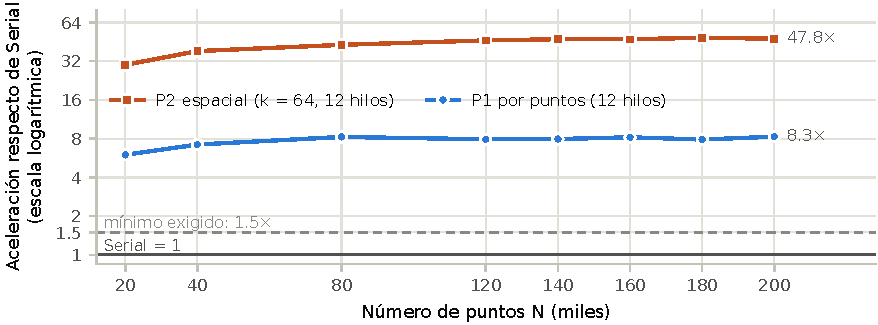
\includegraphics[width=\textwidth]{figuras/fig_speedup_vs_N.pdf}
\caption{Aceleración respecto de Serial al crecer $N$, con configuraciones fijas: P1 con 12 hilos y P2 con $k=64$
y 12 hilos. Cada punto es una razón de medias de diez repeticiones~\eqref{eq:speedup}. El eje vertical es
logarítmico para que la línea base (Serial = 1) y el mínimo exigido (1.5) se lean junto a valores cercanos a 50.}
\label{fig:speedupN}
\end{figure}

\paragraph{Aceleración frente al número de puntos.} Ambas versiones aceleran en todos los tamaños y superan con
amplitud el mínimo de 1.5 (Figura~\ref{fig:speedupN}): P1 va de 5.99 ($N=20{,}000$) a 8.29 ($N=200{,}000$) y P2, de
29.92 a 47.77, entre 5.0 y 6.2 veces más rápido que P1 en cada tamaño. P1 se estabiliza desde 80,000 puntos y P2 desde 120,000; con menos, cada ejecución paralela dura milisegundos (P2: 2.9\,ms con $N=20{,}000$) y es de esperar que
pesen más los costos fijos.

\begin{figure}[t]
\centering
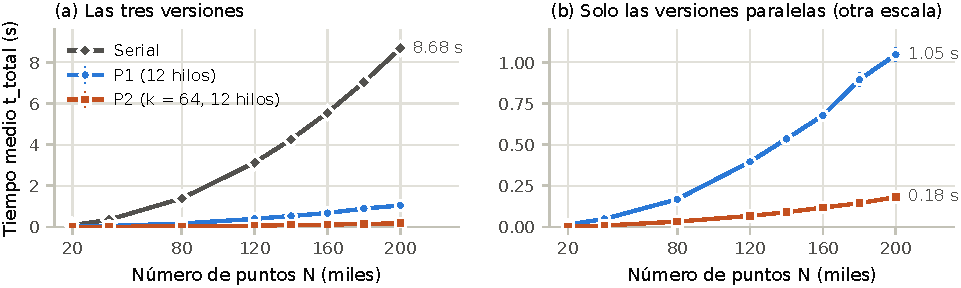
\includegraphics[width=\textwidth]{figuras/fig_tiempo_vs_N.pdf}
\caption{Tiempo medio $T_{\mathrm{total}}$ frente a $N$ con las configuraciones de la Figura~\ref{fig:speedupN}. El
panel (b) repite P1 y P2 en otra escala para distinguirlos. Las barras de error ($\pm1$ desviación estándar) casi
no se ven porque son pequeñas.}
\label{fig:tiempoN}
\end{figure}

\paragraph{Tiempo frente al número de puntos.} Con $N=200{,}000$ (Figura~\ref{fig:tiempoN}) Serial tarda 8.68\,s,
P1 1.05\,s y P2 0.18\,s. Al multiplicar $N$ por 10 el tiempo serial se multiplica por 99, consistente con los $N^2$
pares del Paso~1, aunque ocho tamaños no bastan para afirmar una complejidad asintótica.

\begin{figure}[t]
\centering
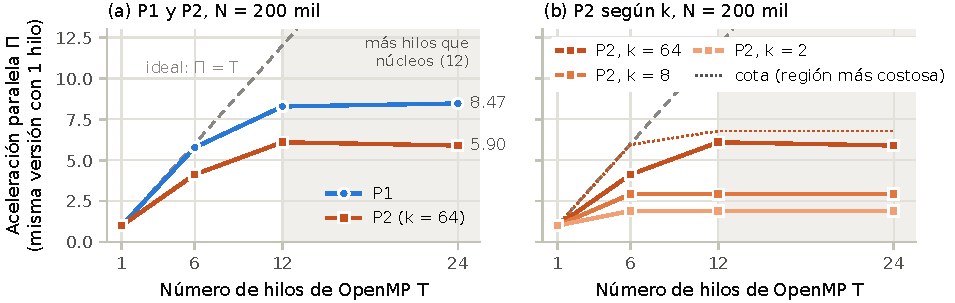
\includegraphics[width=\textwidth]{figuras/fig_escalamiento_hilos.pdf}
\caption{Escalamiento con hilos para $N=200{,}000$, medido con la aceleración paralela
$\Pi(T)=\overline T(1)/\overline T(T)$ de cada versión contra sí misma con un hilo (P2 con $k$ fijo), que aísla el
efecto de los hilos. Línea discontinua: referencia ideal $\Pi=T$; zona gris: más hilos que núcleos. En (b), las
líneas punteadas son la cota que impone la región más costosa si el tiempo fuera proporcional a los pares y los
núcleos fueran idénticos (Sección~\ref{sec:amdahl}).}
\label{fig:hilos}
\end{figure}

\begin{table}[t]
\centering\small
\caption{Escalamiento con hilos para $N=200{,}000$ (Serial: $8.6758\pm0.0161$\,s, CV 0.2\,\%). $\Pi$: aceleración
paralela contra la misma versión con un hilo; $E=\Pi/T$: eficiencia; $S$: aceleración respecto de Serial.}
\label{tab:hilos}
\begin{tabular}{@{}r rrrr c rrrr@{}}
\toprule
 & \multicolumn{4}{c}{P1} & & \multicolumn{4}{c}{P2, $k=64$}\\
\cmidrule{2-5}\cmidrule{7-10}
$T$ & media $\pm$ desv. (s) & CV & $\Pi$ & $E$ & & media $\pm$ desv. (s) & CV & $\Pi$ & $S$\\
\midrule
 1 & $8.6696\pm0.0362$ & 0.4\,\% & 1.00 & 1.00 & & $1.1074\pm0.0032$ & 0.3\,\% & 1.00 & 7.83\\
 6 & $1.5011\pm0.0143$ & 1.0\,\% & 5.78 & 0.96 & & $0.2685\pm0.0005$ & 0.2\,\% & 4.12 & 32.31\\
12 & $1.0466\pm0.0433$ & 4.1\,\% & 8.28 & 0.69 & & $0.1816\pm0.0042$ & 2.3\,\% & 6.10 & \textbf{47.77}\\
24 & $1.0236\pm0.0247$ & 2.4\,\% & 8.47 & 0.35 & & $0.1878\pm0.0036$ & 1.9\,\% & 5.90 & 46.19\\
\bottomrule
\end{tabular}
\end{table}

\paragraph{Escalamiento con hilos.} P1 con un hilo tarda lo mismo que Serial (razón 0.999), así que su aceleración es
puramente paralela (Figura~\ref{fig:hilos}a, Tabla~\ref{tab:hilos}): $\Pi=5.78$ con 6 hilos (eficiencia 0.96), 8.28
con 12 y 8.47 con 24. De 6 a 12 hilos se gana mucho menos que de 1 a 6. Hipótesis compatibles, no demostradas: (a)
los cuatro núcleos de eficiencia son más lentos y, con \code{schedule(static)}, cada hilo recibe el mismo número de
puntos, así que los lentos marcan el final (compatible con que \code{dynamic,64} fuera un 5\,\% más rápido en la
prueba D4); (b) \code{BTLEServer} ocupaba casi un núcleo; (c) recursos compartidos. Con 24 hilos no hay más núcleos;
la ligera mejora podría venir de bloques más chicos que el sistema operativo reequilibra.

P2 con $k=64$ escala peor ($\Pi=6.10$ con 12 hilos), y la Figura~\ref{fig:hilos}b muestra por qué: con $k\le16$,
$\Pi$ es igual con 6, 12 y 24 hilos y queda a 2\,\% o menos de la cota que impone la región más costosa (1.90 frente
a 1.92 con $k=2$; 2.92 frente a 2.97 con $k=8$): una región es una tarea indivisible. Con $k=64$, 12 hilos alcanzan
el 90\,\% de la cota (6.79); con 6 hilos, $\Pi=4.12$ frente a 5.95, señal de que los supuestos del modelo (tiempo
proporcional a los pares, núcleos idénticos) no se cumplen del todo.

\begin{figure}[t]
\centering
\begin{minipage}[t]{0.49\textwidth}
\centering
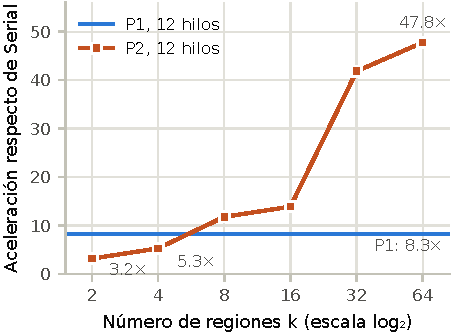
\includegraphics[width=\linewidth]{figuras/fig_speedup_vs_k.pdf}
\caption{Efecto de $k$ con $N=200{,}000$ y 12 hilos: aceleración de P2 respecto de Serial; la línea azul es P1 con
los mismos 12 hilos.}
\label{fig:k}
\end{minipage}\hfill
\begin{minipage}[t]{0.49\textwidth}
\centering
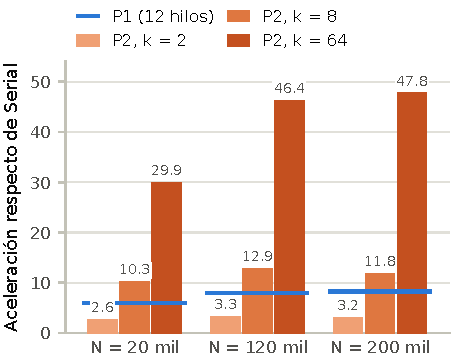
\includegraphics[width=\linewidth]{figuras/fig_barras_N_k.pdf}
\caption{Interacción entre $N$ y $k$ con 12 hilos: aceleración de P2 con un $k$ pequeño, uno intermedio y uno
grande; los segmentos azules marcan a P1 con 12 hilos.}
\label{fig:barras}
\end{minipage}
\end{figure}

\paragraph{Efecto del número de regiones.} Con $N=200{,}000$ y 12 hilos (Figura~\ref{fig:k}), P2 pasa de 3.18
($k=2$) y 5.29 ($k=4$), por debajo de P1 (8.29), a 11.80, 13.90, 41.84 y 47.77 con $k=8$, 16, 32 y 64. Más regiones
actúan por dos vías: menos pares (de $N^2/1.67$ a $N^2/8.13$) y más tareas, cada una más ligera (la más costosa pasa
del 52\,\% al 14.7\,\% de los pares). La segunda explica el salto de $k=16$ a $k=32$: en la cuadrícula $4\times4$ una
celda conserva el 36.5\,\% del trabajo ---más que con $k=8$, por eso $\Pi$ baja de 2.92 a 2.72--- y en la de
$4\times8$ la más pesada baja al 14.5\,\%. Aumentar $k$ no garantiza una mejora: depende de dónde caen las
fronteras respecto de los grupos, y el halo (de 38,791 copias de puntos con $k=2$ a 247,114 con $k=64$) y la
construcción, $O(kN)$, crecen con $k$ (no medimos $k>64$). La Figura~\ref{fig:barras} repite el patrón con 20,000,
120,000 y 200,000 puntos: $k=2$ siempre queda debajo de P1, $k=8$ por encima, y la ventaja de $k=64$ crece con
$N$ (29.9, 46.4 y 47.8).

\paragraph{Por qué P2 superó a P1, y cuándo no.} P1 hace las mismas $N^2$ comparaciones que Serial y las reparte
entre hilos; P2 primero elimina comparaciones con restricciones espaciales y luego reparte las restantes. Con
$N=200{,}000$ y 12 hilos, P2 escala peor ($\Pi=6.10$ contra 8.28), pero evalúa 8.13 veces menos pares y termina 5.76
veces antes. P2 fue más lento que P1 en 48 de las 192 combinaciones $(N,k,T)$ comparables: exactamente las que tienen
$k\in\{2,4\}$ y $T\ge6$. Ahí hay a lo más cuatro tareas, la más pesada con cerca de la mitad del trabajo
($\Pi\le2.04$), y el ahorro de pares (1.67 o 2.63) no compensa la aceleración de P1 con 6 o más hilos (5.6 a 8.5).
Con un hilo, P2 superó a Serial en todas las configuraciones (factor mínimo 1.65). Los mejores resultados fueron 8.53
para P1 ($N=180{,}000$, 24 hilos) y 48.64 para P2 ($N=180{,}000$, $k=64$, 12 hilos).

%======================================================================================================
\section{Ley de Amdahl y descomposición del speedup}\label{sec:amdahl}

La ley de Amdahl~\cite{amdahl1967,diapositivas} acota la aceleración de un trabajo \emph{fijo} cuya fracción $f$ se
divide perfectamente entre $p$ procesadores idénticos, mientras el resto es secuencial:
\begin{equation}\label{eq:amdahl}
  S_{\mathrm{Amdahl}}(p)=\frac{1}{(1-f)+f/p}\;<\;\frac{1}{1-f}.
\end{equation}
Supone además que repartir no cuesta nada; la sincronización, el desbalance de carga y la contención reducen todavía
más la aceleración real~\cite{diapositivas}.

La aceleración total de P2, 47.77 con 12 hilos, no contradice~\eqref{eq:amdahl}: compara dos algoritmos que hacen
distinta cantidad de trabajo. La comparación legítima separa los dos efectos:
\begin{equation}\label{eq:descomp}
  A(N,k)=\frac{\Tser(N)}{\overline T_{P2}(N,k,1)},\qquad
  \Pi(N,k,T)=\frac{\overline T_{P2}(N,k,1)}{\overline T_{P2}(N,k,T)},\qquad
  S_{\mathrm{total}}=A\cdot\Pi .
\end{equation}
$A$ es la ganancia algorítmica (P2 con un hilo frente a Serial) y $\Pi$ la ganancia paralela de la misma
estrategia; solo $\Pi$ debe compararse con Amdahl. Con $N=200{,}000$, $k=64$ y $T=12$: $A=7.83$, $\Pi=6.10$ y
$S_{\mathrm{total}}=47.77$. $A$ es cercano a la reducción de pares, $N^2/\sum_r n_r|L_r|=8.13$; la diferencia se debe casi toda a la construcción (3.5\,\% del tiempo con un hilo), porque sin ella $A$ sería 8.12. Y $\Pi=6.10<12$, como exige
Amdahl. La Tabla~\ref{tab:amdahl} muestra la descomposición para cada $k$.

\begin{table}[t]
\centering\small
\caption{Descomposición $S_{\mathrm{total}}=A\cdot\Pi$ con $N=200{,}000$ y 12 hilos. $N^2/\text{pares}$: reducción de
pares del Paso~1; $1/\smax$: cota de $\Pi$ por la región más costosa, que tiene la fracción $\smax$
(\code{max\_task\_share}) de los pares.}
\label{tab:amdahl}
\begin{tabular}{@{}rrrrrrr@{}}
\toprule
$k$ & regiones con puntos & $N^2/\text{pares}$ & $A$ & $\Pi$ (12 hilos) & $1/\smax$ & $S_{\mathrm{total}}$\\
\midrule
 2 &  2 & 1.67 & 1.67 & 1.90 & 1.92 &  3.18\\
 4 &  4 & 2.63 & 2.62 & 2.02 & 2.04 &  5.29\\
 8 &  8 & 4.06 & 4.04 & 2.92 & 2.97 & 11.80\\
16 & 15 & 5.15 & 5.10 & 2.72 & 2.74 & 13.90\\
32 & 29 & 6.47 & 6.35 & 6.59 & 6.88 & 41.84\\
64 & 55 & 8.13 & 7.83 & 6.10 & 6.79 & 47.77\\
\bottomrule
\end{tabular}
\end{table}

\paragraph{La región más costosa como parte no divisible.} En P2 cada región es una tarea indivisible. Si el tiempo de
una región fuera proporcional a sus pares y los núcleos fueran idénticos, ningún reparto terminaría antes que la
región más pesada, sin importar el número de hilos:
\begin{equation}\label{eq:cota}
  \Pi\;\le\;\frac{\sum_r n_r|L_r|}{\max_r n_r|L_r|}=\frac{1}{\smax}.
\end{equation}
Es una versión del cuello de botella de Amdahl: la región más pesada hace el papel de la parte que no se puede
dividir. Es un modelo idealizado, no una identidad (supone costo uniforme por par, núcleos iguales y reparto
gratuito). Para la Figura~\ref{fig:hilos}b lo evaluamos reconstruyendo, con la regla del programa, el costo de cada
región a partir de los datos (la suma coincide exactamente con \code{pairs\_step1}) y simulando el reparto de mayor a
menor.

\paragraph{P1 y la fracción paralelizable.} Si se despeja $f$ de~\eqref{eq:amdahl} con los $\Pi$ de P1, resulta
$f=0.992$ con 6 hilos y $f=0.959$ con 12. Con una parte secuencial fija, $f$ sería la misma; no lo es, así que la
pérdida depende del hardware ---núcleos heterogéneos, que no equivalen a doce procesadores idénticos--- más que de
una parte secuencial del código. Con estas mediciones no podemos obtener una fracción serial exacta ni atribuir toda
la pérdida de eficiencia a un solo factor.

%======================================================================================================
\section{Limitaciones y prueba de sensibilidad}\label{sec:limites}

Los resultados corresponden a una máquina y a una familia de datos: cuatro grupos gaussianos muy densos (99.9\,\% de
los puntos en $C_1$), lo cual favorece al particionamiento espacial. Para dimensionarlo hicimos una prueba
complementaria, \emph{fuera} de las 2,320 ejecuciones oficiales, con datos sintéticos (\code{results/sensibilidad/}):
uniformes en $[0,1.3]^2$; ``desbalanceados'', con el 80\,\% de los puntos en uno de cinco grupos; y
``concentrados'', con el 99.5\,\% en un cuadrado de $0.06\times0.06$ y pocos puntos lejanos que estiran la caja. Se
midieron tres repeticiones con 12 hilos con una compilación previa a la integración final, cuyo modo espacial es el
algoritmo de P2; las clases y conteos coincidieron con Serial, también con el ejecutable oficial
(Tabla~\ref{tab:sens}).

\begin{table}[t]
\centering\small
\caption{Prueba complementaria de sensibilidad: 40,000 puntos, 12 hilos, media de tres repeticiones (mediciones
provisionales). Con datos uniformes P2 tarda unos 3\,ms, así que esa cifra es poco precisa.}
\label{tab:sens}
\begin{tabular}{@{}lrrrrr@{}}
\toprule
Distribución & Serial (s) & P1 & P2, $k=64$ & $N^2/\text{pares}$ & $\smax$\\
\midrule
Uniforme       & 0.3366 & 8.0 & 121.9 & 36.38 & 0.020\\
Desbalanceada  & 0.3417 & 8.4 &   7.0 &  4.08 & 0.566\\
Concentrada    & 0.3398 & 7.9 &   1.0 &  1.01 & 1.000\\
\bottomrule
\end{tabular}
\end{table}

Las regiones de P2 tienen el mismo tamaño, no el mismo número de puntos. Si casi todos caen en una, apenas se ahorran
comparaciones, una tarea concentra el trabajo y la aceleración desaparece: con datos concentrados P2 quedó en 1.0
mientras P1 conservó unas ocho veces, y en un caso adverso P2 podría ser más lento que Serial porque además paga la
construcción. El P2 por bloques de Mario mantuvo unas ocho veces en las tres
distribuciones, porque no depende de la geometría. Otras limitaciones: $\varepsilon$ y $m$ fijos (un $\varepsilon$
mayor ensancha los halos), hilos sin fijar a núcleos, \code{BTLEServer} activo y un tiempo que excluye la lectura.

%======================================================================================================
\section{Uso responsable y ético de IA generativa}\label{sec:ia}

Seguimos las pautas de IEEE~\cite{ieee-ai} (declarar la herramienta, las partes del trabajo en que se usó y el nivel
de uso) y de Elsevier~\cite{elsevier-ai} (la herramienta no es autora; los autores responden por el contenido).

\paragraph{Herramienta y tareas.} Usamos Claude Opus 5.5 (Anthropic), mediante Claude Code, del 18 al 20 de octubre
de 2026. La bitácora de \code{docs/DECISIONS.md} registra los usos del 18 y 19 de octubre: interpretación del enunciado y plan de
arquitectura (decisiones D1--D12); implementación asistida de \code{src/dbscan.cpp} (Serial, CSV, P1 y P2 espacial),
del \code{Makefile}, de la validación, del ejecutor y del análisis; adaptación y validación del P2 de Mario; y documentación. El 20 de octubre se usó además para redactar este reporte y generar sus figuras con un script desde el CSV oficial.
\pendiente{Confirmar si se usó otra herramienta de IA ---p.\,ej., Codex, previsto en el plan original, o
alguna usada para el código de Mario o para estudiar--- y declararla aquí.}

\paragraph{Aportación del equipo.} El equipo aprobó el plan tras dos rondas de revisión, generó los datos con la
libreta, revisó cada etapa antes de integrarla, decidió qué P2 entregar y ejecutó el experimento oficial en su
computadora. Mario diseñó e implementó la primera P2; su autoría se reconoce en el código, en este reporte y en
\code{experimentos/p2\_xp/}, donde su archivo original se conserva sin cambios.

\paragraph{Verificación.} Ninguna salida de la IA se aceptó por su apariencia: las versiones se contrastaron con la
serial (huellas idénticas en las 2,320 ejecuciones), con casos de clases conocidas, con una referencia en NumPy y con
scikit-learn; se introdujeron errores a propósito para comprobar que las pruebas los detectan; una revisión del
código, también asistida por IA, verificó escrituras disjuntas y barreras; y las cifras del reporte se recalcularon
desde \code{mediciones.csv}.

\paragraph{Declaración.} Durante la preparación de este trabajo, el equipo usó Claude Opus 5.5 para las tareas
descritas. Después de usarla, el equipo revisó y editó el contenido según fue necesario y asume la responsabilidad
total por la corrección del código, las decisiones de diseño, la interpretación de los experimentos y el contenido
de este reporte. \pendiente{Confirmar antes de entregar: ambos integrantes revisaron el reporte completo.}

%======================================================================================================
\section{Conclusiones}\label{sec:conclusion}

Las dos versiones paralelas reprodujeron exactamente la clasificación serial ---clases y conteos de vecinos--- en las
2,320 ejecuciones y superaron con amplitud el mínimo de 1.5. P1, la paralelización directa del algoritmo exhaustivo,
escala casi idealmente hasta 6 hilos y llega a 8.29 con 12; su pérdida de eficiencia posterior es compatible con la
heterogeneidad de los núcleos, aunque no pudimos aislar su causa. P2 fue el más rápido con los datos oficiales
(47.77 con $N=200{,}000$, $k=64$ y 12 hilos) porque combina dos ganancias: evalúa 8.13 veces menos pares gracias a
halos que no pierden vecinos, y reparte las regiones entre hilos ($\Pi=6.10$). Esa ventaja tiene condiciones: con
$k\le4$ P2 fue más lento que P1, su escalamiento está acotado por la región más costosa y, con datos concentrados,
su aceleración desapareció. P2 conviene cuando los puntos se reparten entre muchas regiones, como en los datos del
curso; P1 ofrece un rendimiento más predecible, independiente de la distribución.

\paragraph{Datos experimentales y reproducibilidad.} Las mediciones oficiales están en
\path{results/official/oficial_20261020/mediciones.csv}; en esa carpeta, \path{manifiesto.json} (commit, huellas
SHA-256, máquina, plan y semilla), referencias, bitácora y análisis. Figuras y cifras:
\path{entrega/reporte/generar_figuras.py}. Sensibilidad, validación y P2 por bloques: \path{results/sensibilidad/},
\path{results/validacion/} y \path{experimentos/p2_xp/}.

\begin{thebibliography}{9}\footnotesize\raggedright
\setlength{\itemsep}{0pt}
\bibitem{enunciado} J.~O. Gutiérrez García. \emph{Proyecto Apertura 2026B: DBSCAN} (enunciado) y libreta
\code{DBSCAN\_noise.ipynb}. ITAM, 2026.
\bibitem{diapositivas} J.~O. Gutiérrez García. \emph{Introducción y arquitecturas paralelas} (diapositivas del curso),
ITAM, 2026.
\bibitem{ester1996} M.~Ester, H.-P. Kriegel, J.~Sander y X.~Xu. A density-based algorithm for discovering clusters
in large spatial databases with noise. En \emph{Proc.\ KDD-96}, pp.~226--231, 1996.
\bibitem{amdahl1967} G.~M. Amdahl. Validity of the single processor approach to achieving large scale computing
capabilities. En \emph{AFIPS Spring Joint Computer Conference}, pp.~483--485, 1967.
\bibitem{graham1969} R.~L. Graham. Bounds on multiprocessing timing anomalies. \emph{SIAM J. Appl. Math.},
17(2):416--429, 1969.
\bibitem{sklearn} F.~Pedregosa et al. Scikit-learn: Machine learning in Python. \emph{JMLR}, 12:2825--2830, 2011.
\bibitem{ieee-ai} IEEE. \emph{Author guidelines for AI-generated text}. \url{https://open.ieee.org/author-guidelines-for-artificial-intelligence-ai-generated-text/}.
\bibitem{elsevier-ai} Elsevier. \emph{Generative AI policies for journals}. \url{https://www.elsevier.com/about/policies-and-standards/generative-ai-policies-for-journals}.
\end{thebibliography}

\end{document}
